\section{Intuition Behind Message Aggregation With An Example}\label{sec:motivation_for_aggregation} 

In Chapel, a program's data access patterns and the programmer's choice of data distribution greatly influence the program's runtime and communication behavior. This section presents an example of a Chapel program with affine array accesses that can benefit from message aggregation. It also serves to present the intuition behind how modulo unrolling WU will be used in message aggregation. 

The intuition behind why modulo unrolling is helpful for message aggregation in message passing machines is as follows. Message aggregation requires knowledge of precisely which elements must be communicated between locales. Doing so requires a statically disambiguated known locale for every array access, even when that array access refers to a varying address. For example, in a loop $A[i]$ refers to different memory addresses during each loop iteration. Modulo unrolling ensures such a known, predictable locale number for each varying array access. This enables such varying accesses to be aggregated and sent in a single message. We explain our method of doing so in Sections \ref{sec:transformation} and \ref{sec:adaptation_in_chapel}.

\begin{figure}
\begin{center}
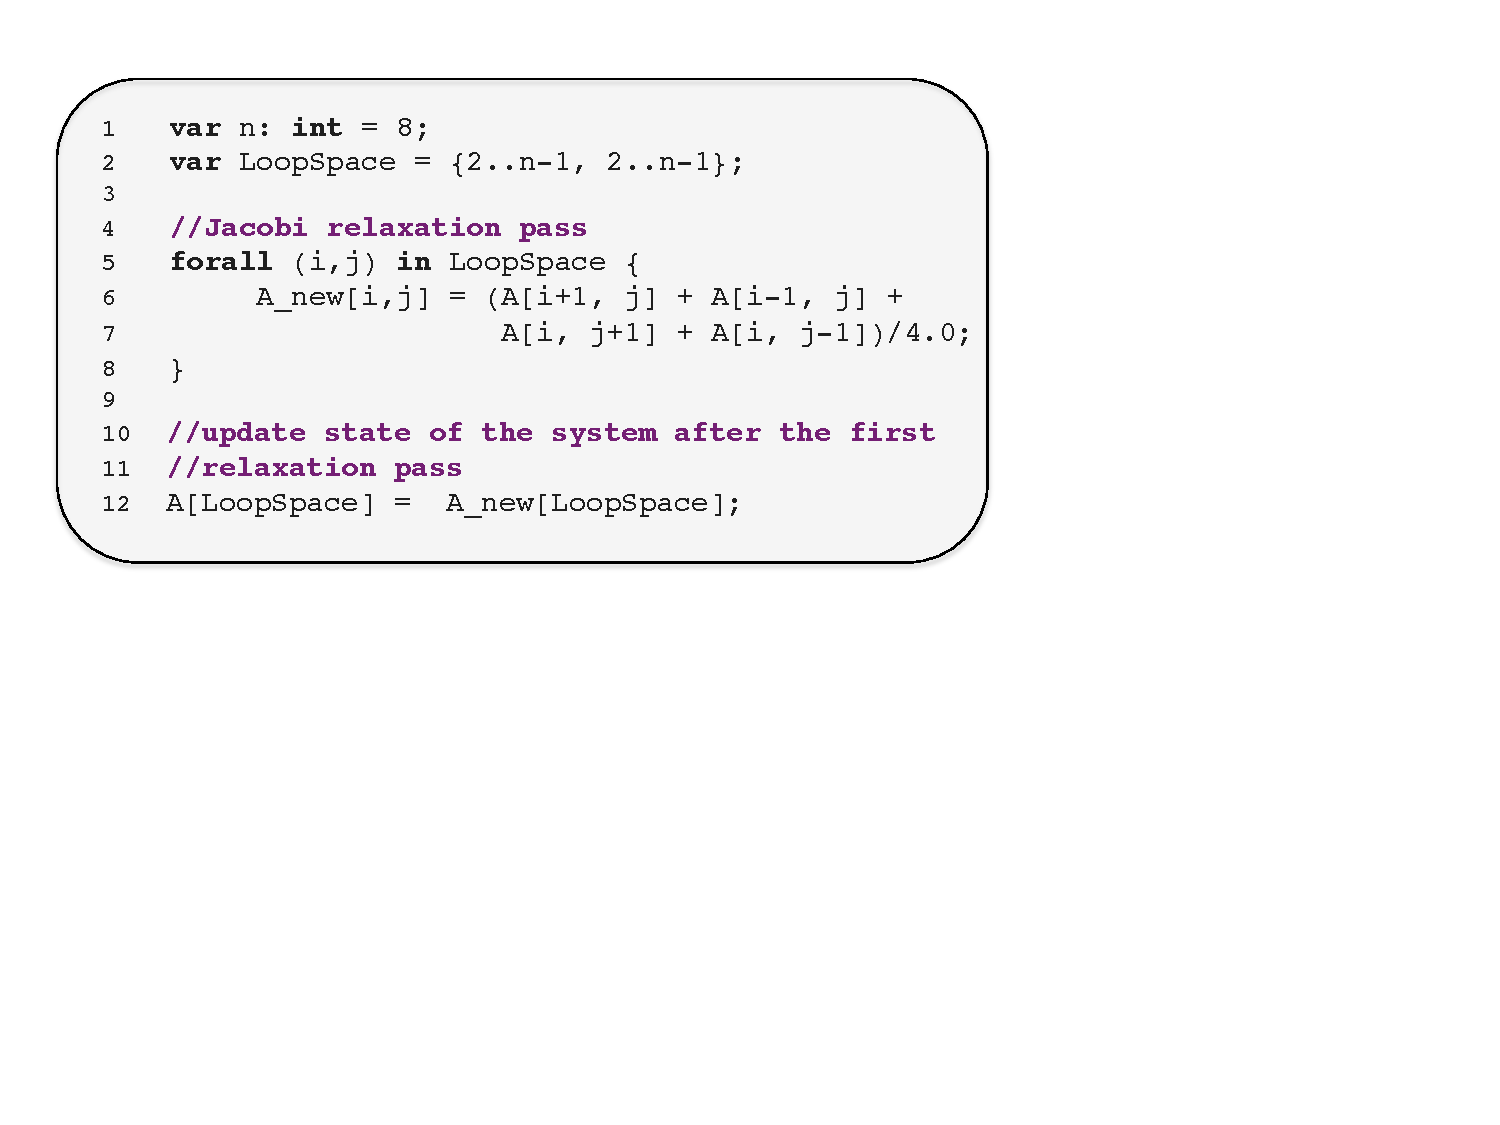
\includegraphics[width=\linewidth]{./Figures/jacobi}
\caption{Chapel code for the Jacobi-2D computation over an 8 x 8 two dimensional array. Arrays $A$ and $A_{new}$ are distributed with a Cyclic distribution and their declarations are not shown. During each iteration of the loop, the current array element $A_{new}[i, j]$ gets the average of the four adjacent array elements of $A[i, j]$.}
\label{jacobi_code}
\end{center}
\end{figure}

\begin{figure}
\begin{center}
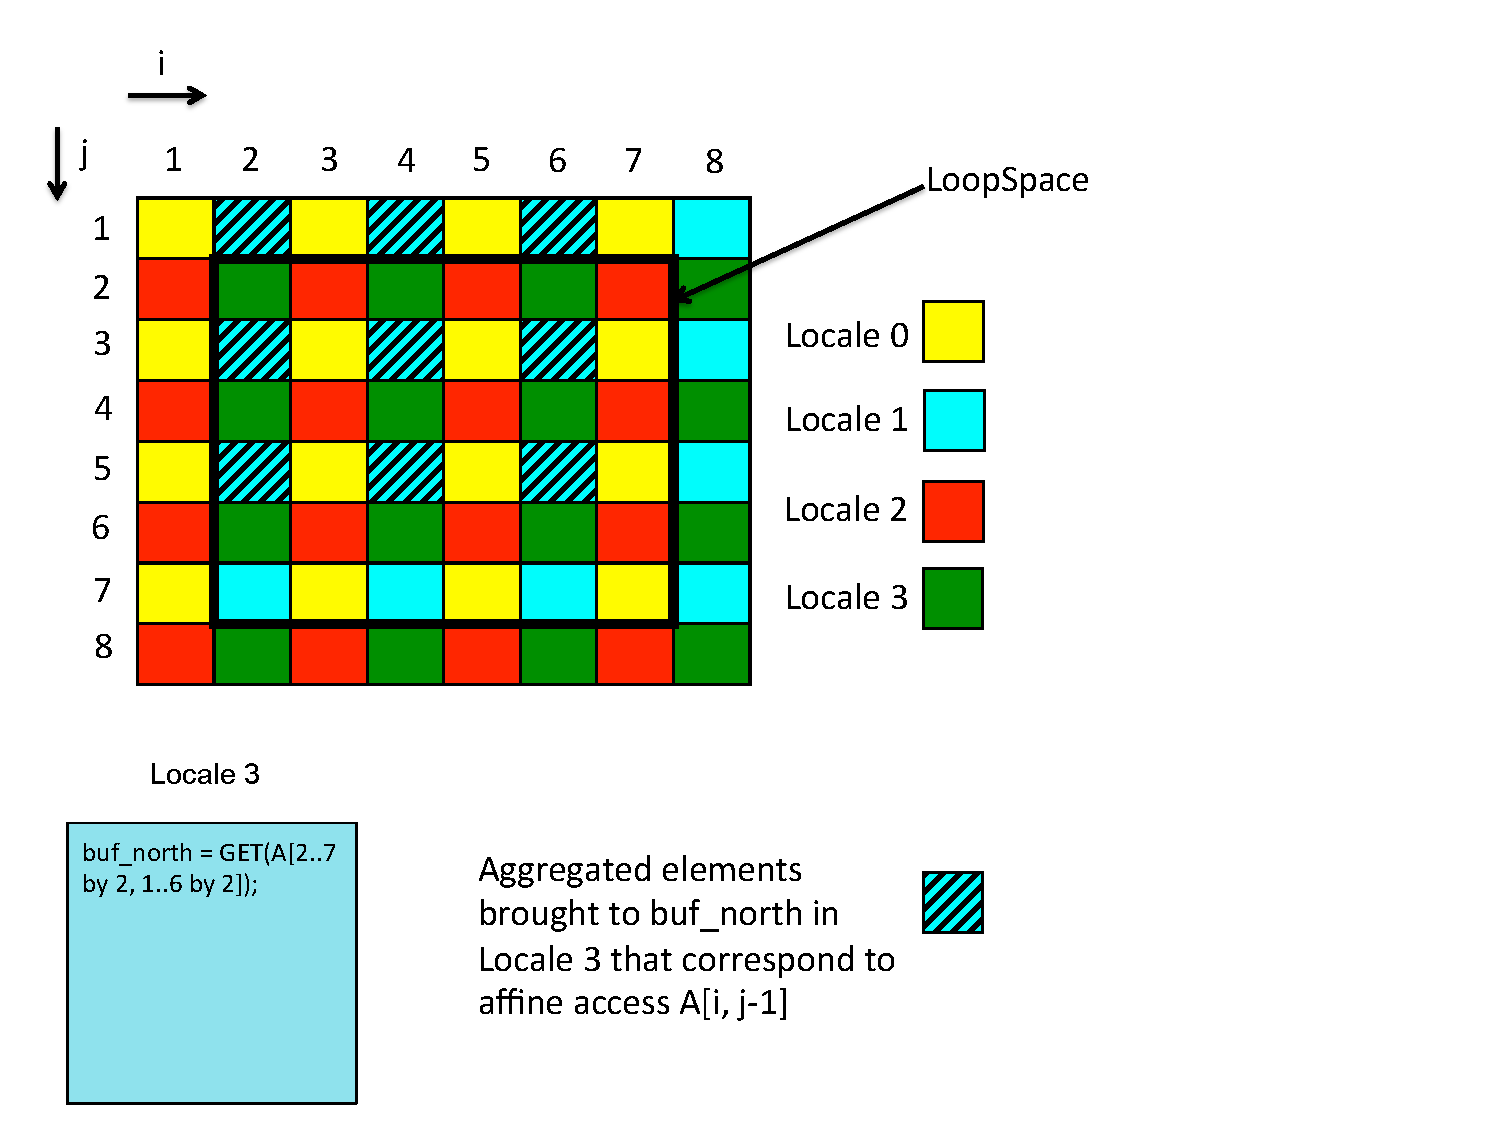
\includegraphics[width=\linewidth]{./Figures/aggregation}
\caption{Illustration of message aggregation for the $A[i, j-1]$ affine array access of the Jacobi-2D relaxation computation with respect to locale 3. The region \textit{LoopSpace} follows from Figure \ref{jacobi_code}. The striped squares are the elements of $A$ that have been aggregated. This same procedure occurs on each locale for each affine array access that is deemed to be remote for all iterations of the loop. For the whole 8 x 8 Jacobi-2D calculation, 144 remote gets containing one element each are necessary without aggregation, but only 16 remote gets containing nine elements each are necessary with aggregation.}
\label{aggregation}
\end{center}
\end{figure}

Consider the Chapel code for the Jacobi-2D computation shown in Figure \ref{jacobi_code}, a common stencil operation that computes elements of a two-dimensional array as an average of that element's four adjacent neighbors. We assume that arrays $A$ and $A_{new}$ have already been distributed using a Cyclic distribution over four locales. On each iteration of the loop, five array elements are accessed in an affine manner: the current array element $A_{new}[i, j]$ and its four adjacent neighbors $A[i+1, j]$, $A[i-1, j]$, $A[i, j+1]$, and $A[i, j-1]$. The computation will take place on the locale of $A_{new}[i, j]$, the element being written to. If arrays $A$ and $A_{new}$ are distributed with a Cyclic distribution as shown in Figure \ref{cyc_dist}, then it is guaranteed that $A[i+1, j]$, $A[i-1, j]$, $A[i, j+1]$, and $A[i, j-1]$ will not reside on the same locale as $A_{new}[i, j]$ \textbf{for all iterations of the loop}. Therefore, these remote elements need to be transferred over to $A_{new}[i, j]$'s locale in four separate messages during every loop iteration. For large data sets, transferring four elements individually per loop iteration drastically slows down the program because the message overhead is incurred many times. 

We observe that message aggregation of remote data elements is possible over the entire loop for the Jacobi-2D example. Aggregation will reduce the number of times the message overhead is incurred during the loop. When the data is distributed using a Cyclic distribution, all array accesses (including remote accesses) exhibit a predictable pattern of locality. 

Figure \ref{aggregation} illustrates this pattern in detail for loop iterations that write to locale 3. During these iterations ($(i, j) = (2, 2), (i, j) = (4, 2)$, etc.), there are two remote accesses from locale 1 and two remote accesses from locale 2. The remote accesses from locale 1 correspond to the $A[i, j+1]$, and $A[i, j-1]$ affine array accesses in Figure \ref{jacobi_code}. If we highlight all the remote data elements corresponding to the $A[i, j-1]$ access that occur for loop iterations that write to locale 3, we end up with the array slice $A[2..7$ $by$ $2, 1..6$ $by$ $2]$, which contains the striped elements in Figure \ref{aggregation}. This array slice can be communicated from locale 1 to a buffer on locale 3 before the loop executes in a single message. Then, during the loop, all $A[i, j-1]$ accesses can be replaced with accesses to the local buffer on locale 3. 

The previous paragraph showed how aggregation occurs for the $A[i, j-1]$ affine array access on loop iterations that write to locale 3. This same procedure applies to the other three remote accesses for locale 3. In addition, this same procedure applies to loop iterations that write to the remaining locales. Finally, we claim that this optimization can also be applied to the Block Cyclic distribution, as the data access pattern is the same for elements in the same position within a block. 

In this example, we chose to perform message aggregation with respect to the element that is written to during the loop. However, this is not always the best choice for all programs. To get better communication performance, we would like to assign loop iterations to locales with the most affine array accesses that are local. The result of this scheme is that elements that are written to during the loop may be the ones that are aggregated before the loop. If so, it is necessary to write these elements from the local buffers back to their remote locales. This is done in a single aggregate message after the loop body has finished.\footnote{In Chapel, the programmer has some control over assigning loop iterations to locales. Therefore, our optimizations uses the programmer's assignment of loop iterations to locales when performing message aggregation.} 

If arrays $A$ and $A_{new}$ are instead distributed using Chapel's Block or Block Cyclic distributions as shown in Figure \ref{block_dist} and Figure \ref{block_cyc_dist} respectively, the program will only perform remote data accesses on iterations of the loop where element $A_{new}[i, j]$ is on the boundary of a block. As the block size increases, the number of remote data accesses for the Jacobi-2D computation decreases. For the Jacobi-2D computation, it is clear that distributing the data using Chapel's Block distribution is the best choice in terms of communication. Executing the program using a Block distribution will result in fewer remote data accesses than when using a Block Cyclic distribution. Similarly, executing the program using a Block Cyclic distribution will result in fewer remote data accesses than when using a Cyclic distribution. 

It is important to note that the Block distribution is not the best choice for all programs using affine array accesses. Programs with strided access patterns that use a Block distribution will have poor communication performance because accessed array elements are more likely to reside outside of a block boundary. For these types of programs, a Cyclic or Block Cyclic distribution will perform better. Section \ref{sec:data_distributions} explained several reasons why the programmer may have chosen a Cyclic or Block Cyclic distribution.

\begin{comment}
When $(i, j) = (2, 2)$, $A_{new}[2, 2]$ resides on locale 3. $A[2, 1]$ corresponds to the $A[i, j-1]$ access during this iteration, and it resides remotely on locale 1. If we now look at the next iteration where $A_{new}[i, j]$ resides on locale 3 (the next cycle, which is $(i, j) = (4, 2)$), we see that $A[4, 1]$ also resides on locale 1. We notice a pattern that all remote data accesses with respect to locale 3 corresponding to the $A[i, j-1]$ access in the loop \textbf{form an array slice $A[2..7$ $by$ $2, 1..6$ $by$ $2]$}, which we can aggregate with a single GET call and bring into $buf$\_$north$ on locale 3 before the loop begins. The array slice contains strided accesses of 2 in both the $i$ and $j$ dimensions, denoted using the Chapel keyword \textit{by} within the array slice. 
\end{comment}




